\documentclass{beamer}

\usepackage{colortbl}
\usepackage{graphicx}
\usepackage{subcaption}

\usepackage{tikz}
\def\checkmark{\tikz\fill[scale=0.4](0,.35) -- (.25,0) -- (1,.7) -- (.25,.15) -- cycle;}

\AtBeginSection[]
{
  \begin{frame}
    \frametitle{Table of Contents}
    \tableofcontents[currentsection]
  \end{frame}
}

\newcommand{\source}[1]{\begin{textblock*}{4cm}(8.7cm,8.6cm)
    \begin{beamercolorbox}[ht=0.5cm,right]{framesource}
        \usebeamerfont{framesource}\usebeamercolor[fg]{framesource} Source: {#1}
    \end{beamercolorbox}
\end{textblock*}}

\usetheme{Madrid}
\usecolortheme{beaver}
% \setbeamercovered{transparent}

\author{AJ Fagan}
\title{Synergy, Toxicity, Efficacy}
\subtitle{In Vitro Drug Interaction Inference}
\institute{UW Madison - Biostatistics}
\date{August 2024}

\begin{document}

\maketitle


\section{Introduction}

\begin{frame}[t]{Introduction}

    \begin{block}{Question}
        How do we quantify the effectiveness of drug combinations in a drug discovery context?
    \end{block}
    \vfill
    Drug combinations serve myriad purposes
    \begin{center}
    \begin{itemize}[<+->]\color{gray}
        \item \color<.>{black} Overcoming resistance
        \item \color<.>{black} Increasing effectiveness
        \item \color<.>{black} Reducing toxicity
        \item \color<.>{black} Repurposing existing drugs
    \end{itemize}
    \end{center}

\end{frame}

\begin{frame}{Example: Atovaquone-Brusatol}
    \begin{center}
        \includegraphics<1>[width=0.8\textwidth, height=0.8\textheight]{figs/etc.jpg}
        \includegraphics<2>[width=0.8\textwidth, height=0.8\textheight]{figs/etc-ato.png}
        \hspace*{15pt}\hbox{\scriptsize Credit:\thinspace{\scriptsize\itshape biologydictionary.net/electron-transport-chain-and-oxidative-phosphorylation/}}
    \end{center}
\end{frame}

\begin{frame}{Atovaquone-Brusatol (cont'd.) - Nrf2}
    \begin{center}
        \includegraphics<1>[width=0.8\textwidth, height=0.8\textheight]{figs/nrf2-pathway.png}
        \includegraphics<2>[width=0.8\textwidth, height=0.8\textheight]{figs/nrf2-pathway-half-annotated.png}
        \includegraphics<3>[width=0.8\textwidth, height=0.8\textheight]{figs/nrf2-pathway-annotated.png}
        \hspace*{15pt}\hbox{\scriptsize Credit:\thinspace{\scriptsize\itshape The Effect of Nrf2 on Diabetic Complications, Reis et. al., 2016}}
    \end{center}
\end{frame}

\begin{frame}{Atovaquone-Brusatol (cont'd.)}

    \begin{block}{Hypothesis}
        Atovaquone and Brusatol, in combination, will exhibit a synergistic effect in cell mortatility in cancer cell lines.
    \end{block}

    \vfill
    \begin{block}{Test - Nicha Boonpattrawong, Patankar Lab}
        \begin{itemize}
            \item A 96-well plate was populated with the cancer cell line OVCAR3.
            \item Then, the wells were treated with various combinations of Atovaquone, Brusatol, and control (DMSO).
            \item After 72 hours, the plates were fed through a plate-reader that determines the Optical Density (OD) in each well.
        \end{itemize}
    \end{block}

\end{frame}

\begin{frame}{Atovaquone-Brusatol Experimental Design}
    \begin{center}
        Set 1: 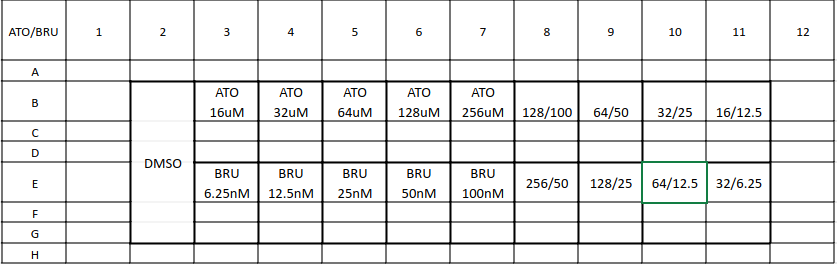
\includegraphics[width=0.8\textwidth, height=0.4\textheight]{figs/set1.png}
        \vfill
        Set 2: 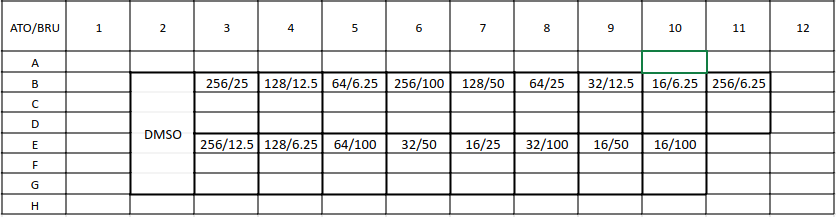
\includegraphics[width=0.8\textwidth, height=0.4\textheight]{figs/set2.png}
    \end{center}
\end{frame}

\begin{frame}{Atovaquone-Brusatol Results}
    \begin{table}
        \centering
        \begin{tabular}{c|c|c|c|c|c|c}
            Ato ($\mu$M)/Bru (nM)   & 0.0  & 6.25 & 12.5 & 25.0 & 50.0 & 100.0  \\\hline
            0.0                     & \cellcolor{ white!00} 2.10 & \cellcolor{  blue!35} 1.73 & \cellcolor{  blue!35} 1.78 & \cellcolor{  blue!35} 1.44 & \cellcolor{  blue!35} 0.95 & \cellcolor{  blue!35} 0.59   \\
            16.0                    & \cellcolor{  blue!35} 1.83 & \cellcolor{yellow!75} 1.67 & \cellcolor{  blue!35} 1.72 & \cellcolor{yellow!75} 1.50 & \cellcolor{yellow!75} 0.98 & \cellcolor{yellow!75} 0.59   \\
            32.0                    & \cellcolor{  blue!35} 0.76 & \cellcolor{  blue!35} 0.75 & \cellcolor{yellow!75} 0.90 & \cellcolor{  blue!35} 0.98 & \cellcolor{yellow!75} 0.84 & \cellcolor{yellow!75} 0.60   \\
            64.0                    & \cellcolor{  blue!35} 0.75 & \cellcolor{yellow!75} 0.74 & \cellcolor{  blue!35} 0.72 & \cellcolor{yellow!75} 0.65 & \cellcolor{  blue!35} 0.60 & \cellcolor{yellow!75} 0.58   \\
            128.0                   & \cellcolor{  blue!35} 0.95 & \cellcolor{yellow!75} 0.91 & \cellcolor{yellow!75} 0.70 & \cellcolor{  blue!35} 0.74 & \cellcolor{yellow!75} 0.69 & \cellcolor{  blue!35} 0.79   \\
            256.0                   & \cellcolor{  blue!35} 1.12 & \cellcolor{yellow!75} 0.89 & \cellcolor{yellow!75} 0.99 & \cellcolor{yellow!75} 0.76 & \cellcolor{  blue!35} 0.94 & \cellcolor{yellow!75} 0.90   \\
        \end{tabular}
        \label{table:ato-bru-mean}
        \caption{
            Mean OD for each Atovaquone/Brusatol dose combination in the OVCAR3 cell line. 
            Blue and yellow highlighted squares are dose combinations found exclusively in Set 1 and 2, respectively.
        }
    \end{table}
\end{frame}

\begin{frame}{Atovaquone-Brusatol Results (cont'd.)}
    \begin{figure}[b]
        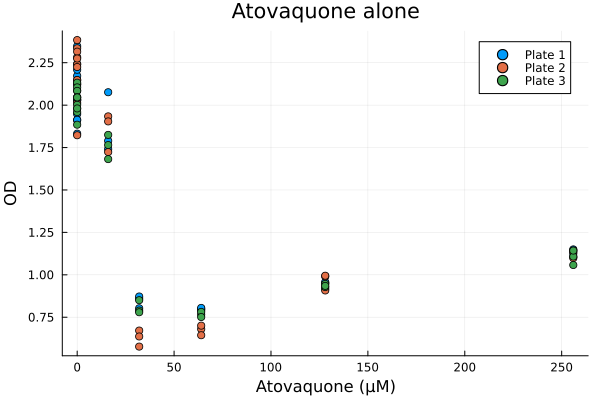
\includegraphics[width=0.9\textwidth]{figs/constant_rate_xto0.0.png}
    \end{figure}
\end{frame}


\section{Modeling Synergy}

\begin{frame}{Synergy}
    Two (or more) drugs can either be \begin{itemize}
        \item Synergistic 
        \item Additive
        \item Antagonistic
    \end{itemize}
   
    \vfill 
    \begin{itemize}
      \item What it means for two drugs to be synergistic or antagonistic seems intuitive.
      \item However, the meaning of drug \textit{additivity} is much less clear, and there are several dozen different definitions.
      \item This makes actually quantifying the notion of synergy and antagonism much more
    \end{itemize}

\end{frame}
\begin{frame}{Example: Atovaquone and Brusatol Inference}
    Atovaquone and Brusatol \begin{itemize}[<+->]\color{gray}
      \item \color<.>{black} had very small \alert{Loewe} synergy scores for small doses of Atovaquone, but ultimately, was not overall statistically significant
      \item \color<.>{black} was statistically significantly antagonistic via \alert{Bliss}/\alert{ZIP} 
      \item \color<.>{black} had several dose-combinations which were statistically significantly \alert{HSA} antagonistic
    \end{itemize}
\end{frame}

\begin{frame}{This is weird}


    \begin{columns}
        \begin{column}{0.7\textwidth}
            \begin{center}
                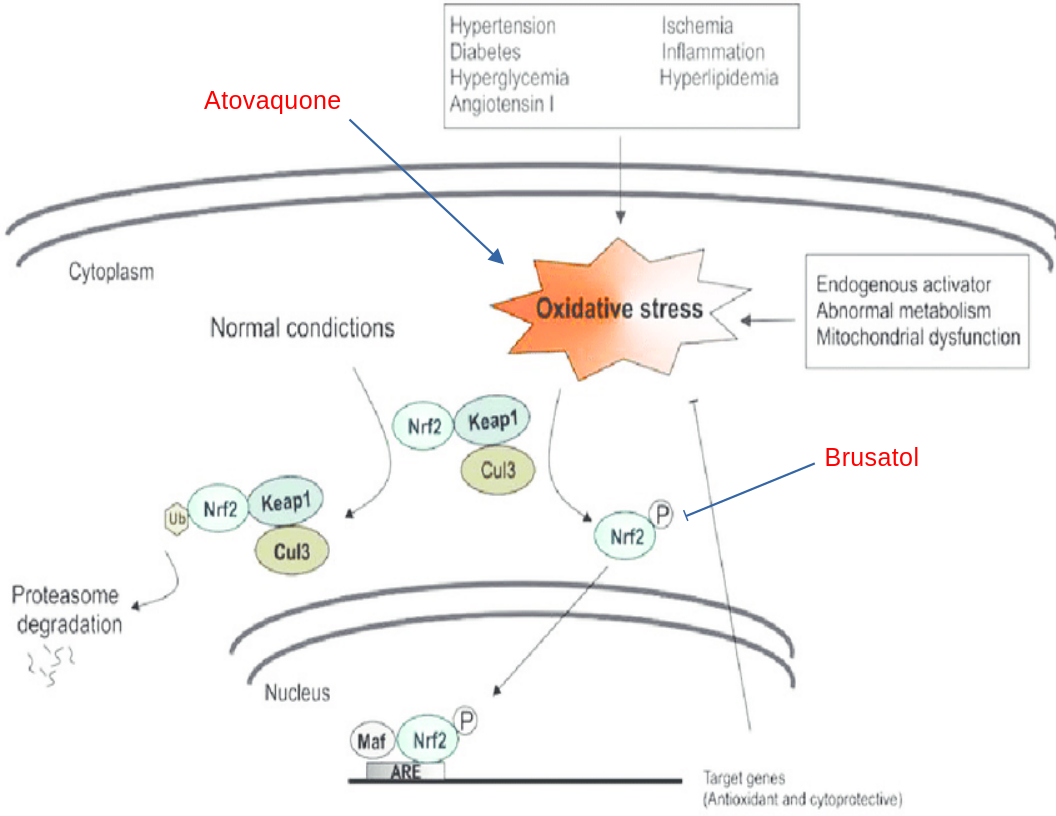
\includegraphics[width = 0.9\textwidth]{figs/nrf2-pathway-annotated.png}


        \hspace*{15pt}\hbox{\scriptsize Credit:\thinspace{\scriptsize\itshape The Effect of Nrf2 on Diabetic Complications, Reis et. al., 2016}}
            \end{center}
        \end{column}
        \begin{column}{0.3\textwidth}
            
            Possible explanations: \begin{itemize}
                \item \alert{Brusatol might need to be introduced first}
                \item Brusatol has other effects
                \item Second pathway
                \item Error
            \end{itemize}
        \end{column}
    \end{columns}
\end{frame}

\section{Efficacy and Toxicity}

\begin{frame}{Goals for Drug Combinations}
    Recall drug combinations goals/promises:
    \begin{itemize}
        \item Overcoming resistance \only<2>{\checkmark}
        \item Increasing effectiveness \only<2>{\checkmark}
        \item \alert<2>{Decreasing toxicity}
        \item Repurposing existing drugs \only<2>{\checkmark}
    \end{itemize}
\end{frame}

\begin{frame}{Relevant XKCD}
    \begin{center}
        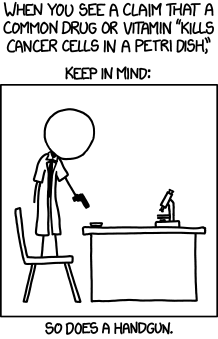
\includegraphics[height=0.7\textheight]{figs/xkcd-cells.png}

        \hspace*{15pt}\hbox{\scriptsize Credit:\thinspace{\scriptsize\itshape XKCD - Cells: https://xkcd.com/1217/}}
    \end{center}
\end{frame}


\begin{frame}{Synergy Can Be Undesirable}
    Synergy tells us we can achieve a similar inhibitory effect using ``less drug''
    \begin{itemize}[<+->]\color{gray}
        \item \color<.>{black} Not, inherently, a beneficial result
        \item \color<.>{black} This effect may be as great or greater in healthy cells 
        \item \color<.>{black} Beaten resistances may be necessary for healthy cells to survive
    \end{itemize}
    \only<4>{
        The ideal drug combination would be synergistic(?), and more potent in cancerous tissue than in healthy.
    }
    \vfill 
    \only<4>{
        \centering
        A more general metric would consider \alert{synergy}, while comparing \alert{efficacy} and \alert{toxicity}.
    }
\end{frame}

\begin{frame}{U-shaped Dose Response Curves}
    \centering
    % 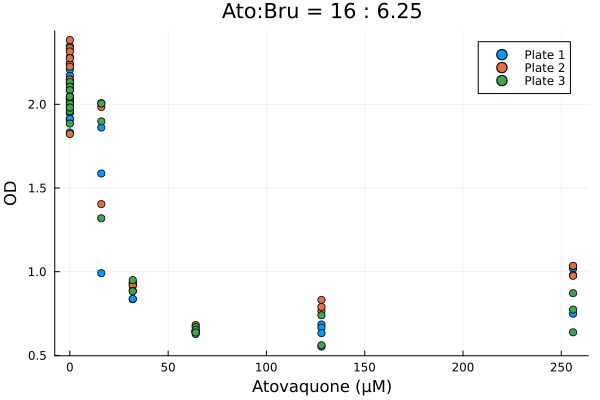
\includegraphics[width=0.8\textwidth]{figs/constant_rate_16to6.25.png}
    \only<1>{
        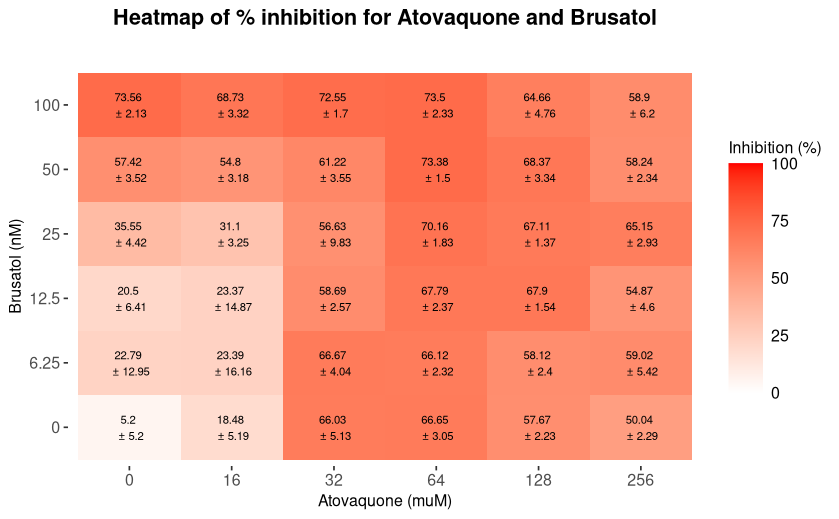
\includegraphics[width=0.9\textwidth]{figs/response-heatmap-all.png}
    }
    \only<2>{
        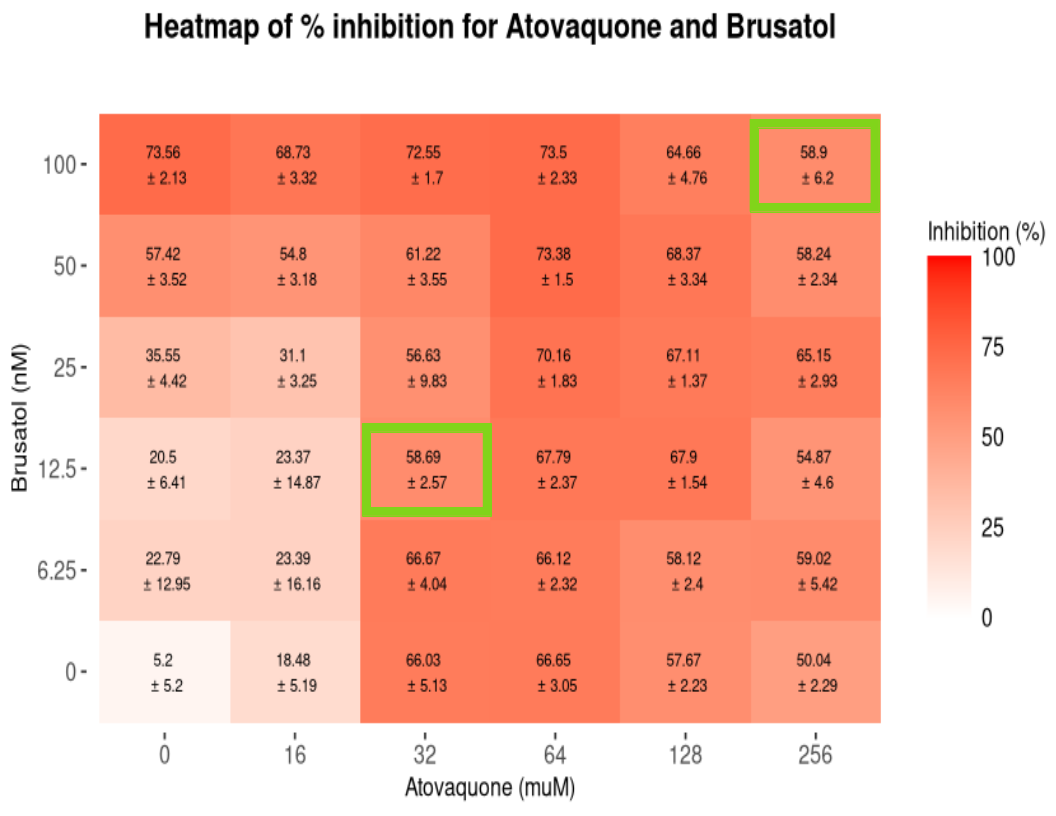
\includegraphics[width=0.8\textwidth]{figs/response-heatmap-all-annotated.png}
    }
\end{frame}


\begin{frame}{DrugCombDB - Cancer Cell Lines}
    DrugCombDB, and similar databases, contain no data on healthy tissue.
    \begin{center}
        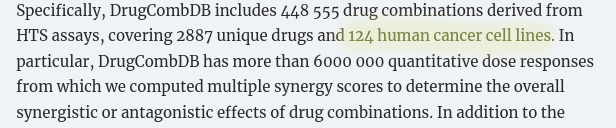
\includegraphics[width = 0.9\textwidth]{figs/drug-comb-cancer-cells.png}
    \end{center}
\end{frame}

\begin{frame}{SynToxProfiler}
    \centering
    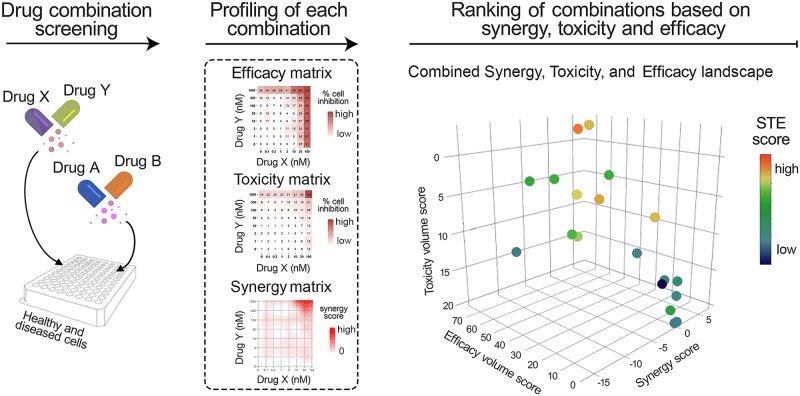
\includegraphics[width=0.9\textwidth]{figs/syntoxprofiler.jpg}

    \hspace*{15pt}\hbox{\scriptsize Credit:\thinspace{\scriptsize\itshape Ianevski et. al., 2020}}
\end{frame}


\begin{frame}{SynToxProfiler Methods}
    Calculate (normalized) volume under 
    \begin{itemize}
        \item $E_{AB}$: Efficacy curve (cancer tissue)
        \item $T_{AB}$: Toxicity curve (healthy tissue)
        \item $S_{AB}$: Synergy curve (cancer tissue)
    \end{itemize}
    \vfill
    For each combination, calculate and rank by STE score 
    \[
        {\rm STE}_{AB} = \frac{{\rm rank}(S_{AB}) + {\rm rank}(E_{AB} - T_{AB})}{2N}
    \]
\end{frame}

\begin{frame}{SynToxProfiler Test}
  TODO: Discuss the course project I did for Christina's course.

  \vfill

  Moral: SynToxProfiler screened out at least one drug combination that had a very high synergy but very poor selective efficacy, and that combination was found to be overly toxic in clinical trials.
\end{frame}

\section{Proposed Research Topics}

\subsection{Synergy Score Aggregation}

\begin{frame}
  \frametitle{Synergy Score Aggregation}
  Many of the most popular methods of determining synergy are \textit{non-parametric}, which means we estimate a \alert{different synergy score for each dose-combination}.

  \vfill
  To make a decision of additive vs synergistic vs antagonistic, we need to aggregate this 3D data into a single value.
  \begin{enumerate}
    \item Pick your favorite (common in non-methods literature)
    \item Sum all the synergy scores 
    \item TODO: others?
  \end{enumerate}

  These have problems:
  \begin{enumerate}
    \item Ignores opposite effects elsewhere, allows for biased selection of ``favorite''.
    \item Removes relevant features of the 3D curve\begin{itemize}
	\item For example, do we see synergy in high dose of A and low dose of B, but antagonism when switched?
      \end{itemize}
  \end{enumerate}
\end{frame}

\begin{frame}
  \frametitle{Synergy Score Aggregation}
  \begin{center}
    {\Large{\alert
      {Is there a better method of aggregating synergy scores?}}
    }
  \end{center}
  \vfill
  \begin{enumerate}
    \item Generate both a synergy ($\max\{f, 0\}$) and an antagonism ($\min\{f, 0\}$) score separately. 
      \begin{itemize}
	\item Doesn't let antagonistic regions drag down synergistic regions
	\item May allow a combination to be all three of additive, synergistic, and antagonistic
      \end{itemize}
    \item Look for \textit{large, connected} dose-combination regions with high synergy.
      \begin{itemize}
	\item Hopes to make claims such as ``high doses of A react synergistically with low doses of B''.
      \end{itemize}
  \end{enumerate}
\end{frame}


\begin{frame}{Example: Loewe Synergy for Atovaquone-Brusatol}
    \centering
    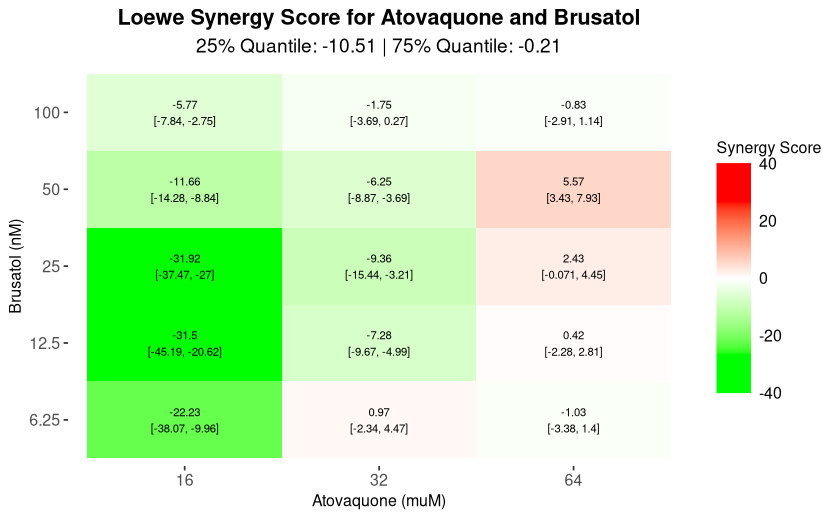
\includegraphics[width=0.9\textwidth]{figs/loewe-heatmap.png}
\end{frame}

\subsection{Network-Based Synergy}

\begin{frame}
  \frametitle{Network Analysis of Synergy}
  Many modern methods (TODO: citations) incorporate gene or protein interaction networks to supplement synergy analysis through, e.g.
  \begin{itemize}
    \item Prediction, especially in HTS contexts
    \item Explaining synergy outcomes
  \end{itemize}
  
  \vfill 
  However, to the best of my knowledge, nobody has ever defined \alert{synergy \textit{within} a network}.
\end{frame}


\begin{frame}
  \frametitle{Synergy within Networks}

  Such a method would seek to find subnetworks of, say, a GRN that are ``especially (in)active'' in the presence of the drug combination than would be expected if there drugs didn't interact.

  \vfill
  Potential benefits:
  \begin{enumerate}
    \item Networks can inherently convey information on relationships between drugs 
    \item May answer more pertinent questions --- synergism within a subnetwork similar to a gene set can enable qualitative analysis of the potential therapeutic benefit of the combination 
    \item Networks are cool and flashy
  \end{enumerate}
  Cons:
  \begin{enumerate}
    \item More expensive and time-consuming analyses would be needed, such as RNASeq.
    \item TODO: Others?
  \end{enumerate}
\end{frame}

 
\subsection{Non-monotonic Dose-Response Curves}

\begin{frame}
  \frametitle{Non-monotonic Dose-Response Curves}

    \centering
    % 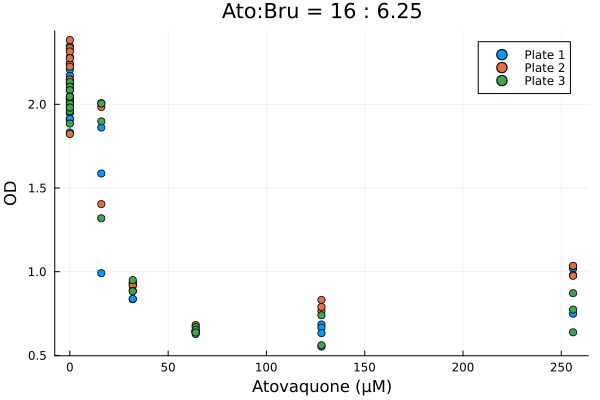
\includegraphics[width=0.8\textwidth]{figs/constant_rate_16to6.25.png}
    
    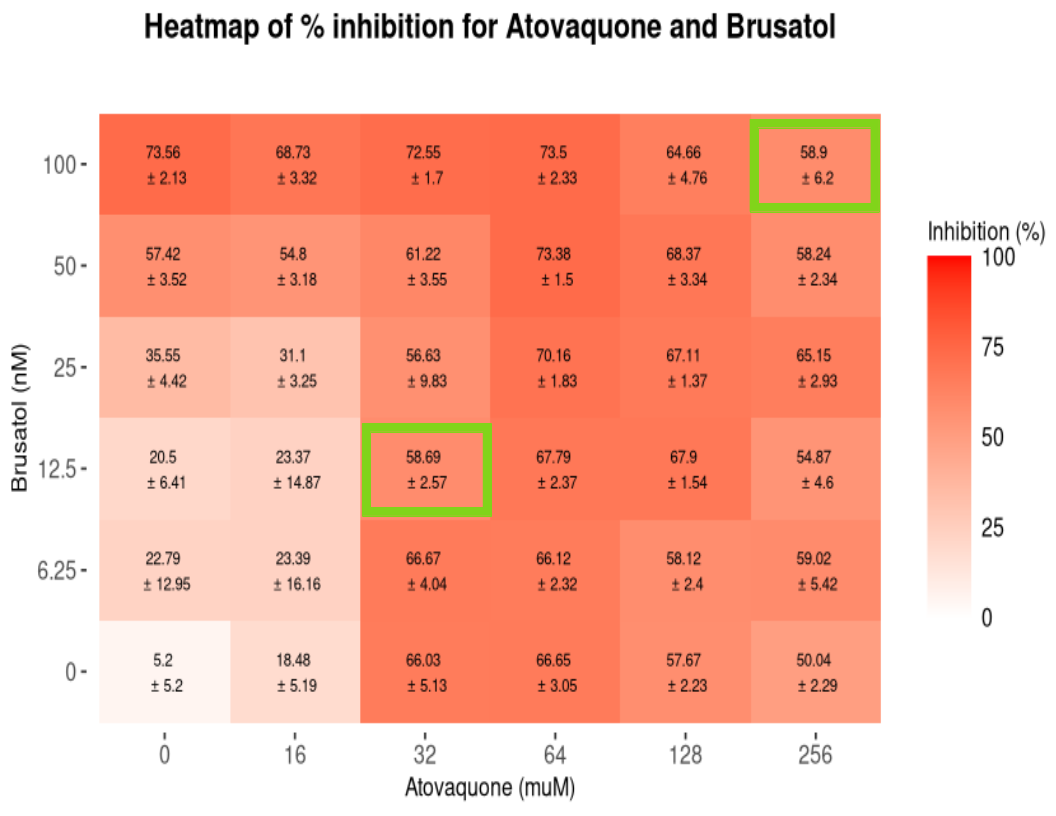
\includegraphics[width=0.8\textwidth]{figs/response-heatmap-all-annotated.png}
\end{frame}


\begin{frame}[allowframebreaks]
    \frametitle{References}
    \bibliographystyle{amsalpha}
    \bibliography{main.bib}
    \nocite{CHENG2021111652}
    \nocite{CHOU1976253}
    \nocite{Ianevski2020-sv}
    \nocite{drugcombdb}
    \nocite{synergyfinder}
\end{frame}

\section{Supplementary}


\subsection{Monotherapeutic Dose-Response Curves}

\begin{frame}{Median-Effect Equation}

    \begin{definition}[Median-Effect Equation (MEE)]
        \[
            \log\frac{f_a}{1 - f_a} = n\log D - n \log D_m,
        \]
        where
        \begin{itemize}
            \item $f_a$ is the \textit{fraction effected} of a receptor
            \item $D$ is the dose of ligand
            \item $D_m$ is the \textit{median effect dose}
            \item $n$ is the \textit{Hill coefficient}
        \end{itemize}
    \end{definition}

    \begin{itemize}
        \item Governs how concentration of ligand influences the proportion of receptors effected
        \item Derived by Ting-Chao Chou in 1976 from the mass effect law
        \item Provides a nice justification for linear models
    \end{itemize}
\end{frame}

\begin{frame}{Atovaquone/Brusatol MEE Curves}
    Define \[
        Survival_{ijk} = OD_{ijk} / \max_{i'}\{OD_{i'jk}\}
    \]
    for the $i$th well in the $j$th plate and $k$th set.
    \begin{figure}
        \centering
        \begin{subfigure}{0.5\textwidth}
            \centering
            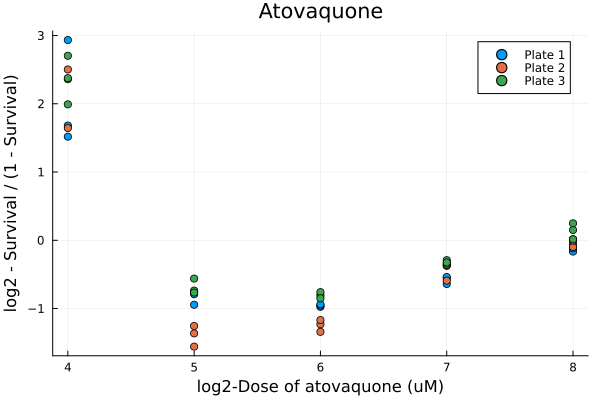
\includegraphics[width=0.9\textwidth]{figs/ato-survival.png}
        \end{subfigure}%
        \begin{subfigure}{0.5\textwidth}
            \centering
            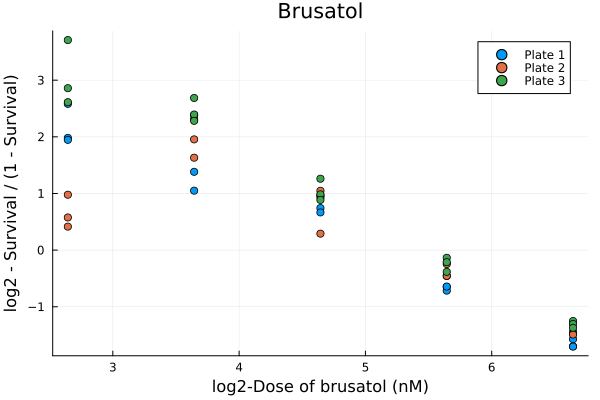
\includegraphics[width=0.9\textwidth]{figs/bru-survival.png}
        \end{subfigure}
    \end{figure}
\end{frame}

\begin{frame}{4 Parameter Logistic Regression}
    \begin{Definition}[4 Parameter Logistic (4PL) Curve]
        \[
            f(D) = \eta_0 + \frac{\eta_f - \eta_0}{1 + \left(\frac{D}{D_m}\right)^{-n}},
        \]
        where \begin{itemize}
            \item $\eta_0$ is the \textit{minimal effect}
            \item $\eta_f$ is the \textit{maximal effect}
        \end{itemize}
    \end{Definition}
    \vfill
    \begin{itemize}
        \item Generalizes the Hill equation 
        \item Enables minimal and maximal effects 
        \item No longer has a nice linear form 
        \item Still asserts monotonicity
    \end{itemize}
\end{frame}

\begin{frame}{Atovaquone/Brusatol 4PL Curves}
    \begin{figure}
        \centering
        \begin{subfigure}{0.5\textwidth}
            \centering
            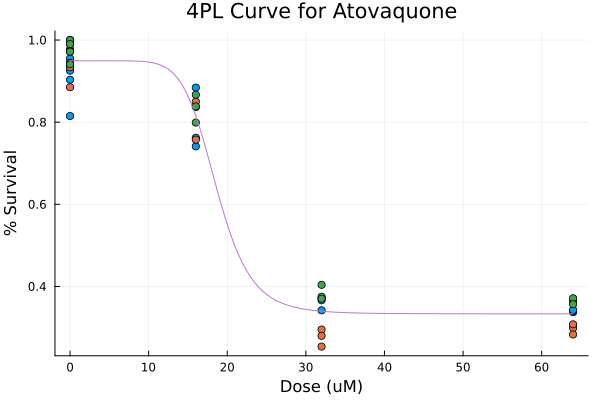
\includegraphics[width=0.9\textwidth, height = 0.6\textheight]{figs/ato4pl.png}
        \end{subfigure}%
        \begin{subfigure}{0.5\textwidth}
            \centering
            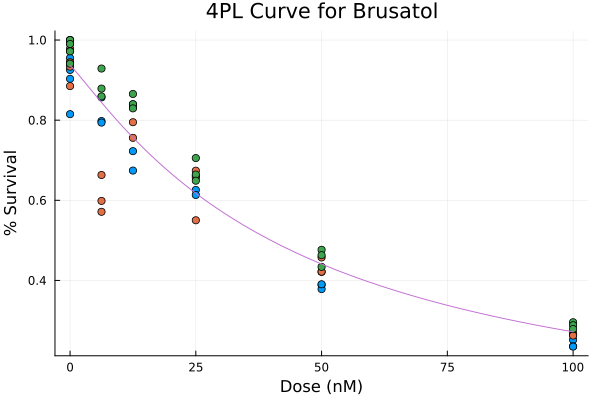
\includegraphics[width=0.9\textwidth, height = 0.6\textheight]{figs/bru4pl.png}
        \end{subfigure}
    \end{figure}
\end{frame}


\begin{frame}{Loewe Additivity}
    \begin{definition}[Loewe Additivity]
        We say that two drugs, $A$ and $B$ are \alert{Loewe Additive} if \[
            \frac{\lambda D}{f_A^{-1} (f_{AB, \lambda}(D))} + \frac{(1 - \lambda) D}{f_B^{-1} (f_{AB, \lambda}(D))} = 1.
        \]
    \end{definition}
    \vfill 
    \begin{itemize}
        \item Most common method of defining synergy
        \item Passes the \alert{Sham-experiment test} - a drug acts additively with itself
        \item The LHS is referred to as the \textit{Combination Index}
        \item Can be undefined for some $D$
    \end{itemize}
\end{frame}

\begin{frame}{Isoboles}
    Loewe additivity results in linear \textit{Isoboles}.
    \begin{itemize}
        \item Atovaquone $D_m$ = 18.62 $\mu$M
        \item Brusatol $D_m$ = 45.10 nM
    \end{itemize}
    \begin{center}
        \only<1>{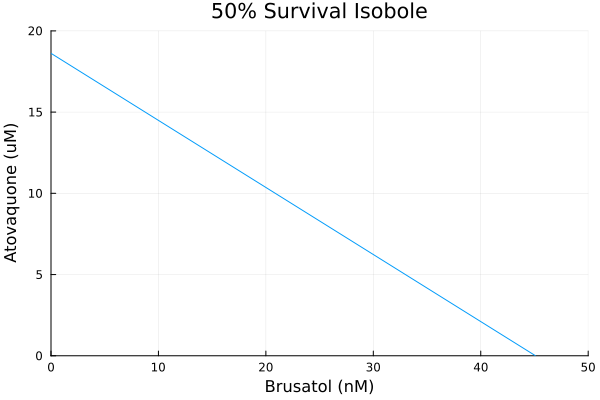
\includegraphics[width=0.8\textwidth]{figs/isobole50.png}}
        \only<2>{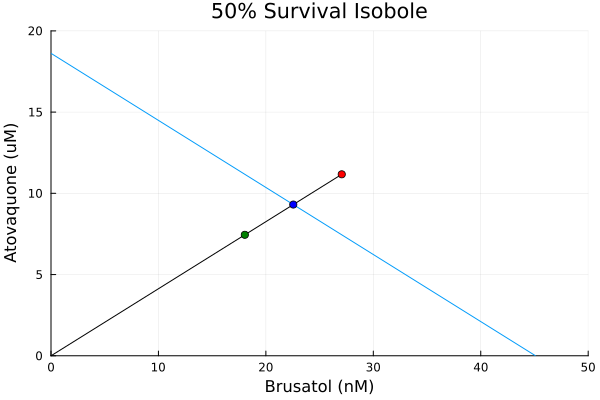
\includegraphics[width=0.8\textwidth]{figs/isobole50-annotated.png}}
    \end{center}

\end{frame}

\begin{frame}{Chou-Tulalay Combination Index Method}
    \begin{Definition}[Combination Index]
        \[
            CombInd = \frac{\lambda D}{f_A^{-1} (f_{AB, \lambda}(D))} + \frac{(1 - \lambda) D}{f_B^{-1} (f_{AB, \lambda}(D))}
        \]
    \end{Definition}
    \begin{center}
        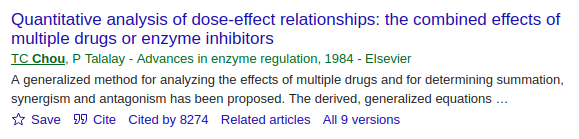
\includegraphics[width=0.8\textwidth]{figs/cimethod-scholar.png}
    \end{center}

    \vfill 

    \begin{itemize}
        \item Assumes $AB$ acts as a third drug, thus, $f_{AB, \lambda}(D)$ should follow a MEE
        \item Generates a value for CombInd at each effect level in $(0,1)$
        \item Produces biased results
    \end{itemize}
\end{frame}

\begin{frame}{Bias in Chou-Tulalay Combination Index}
    \begin{center}
        \large \underline{Toy Example}
    \end{center}
    \only<1>{
    Suppose we have two drugs, $A, B$ that follow MEE curves, are truly Loewe additive, and we know that 
    \begin{itemize}
        \item $n_A = 1.9$, $n_B = 0.7$
        \item $D_{mA} = 27.0$ nM, $D_{mB} = 100.0$ nM
    \end{itemize}
    and, further, suppose we observe the \alert{true} inhibition, $f_{AB, \lambda}(D)$ for
    \begin{itemize}
        \item $\lambda = 1/11$
        \item $D \in \{11, 22, 44, 66, 88, 110\}$ nM
    \end{itemize}
    }

    \only<2>{
        We would observe the following Dose-Response curve:
        \begin{center}
            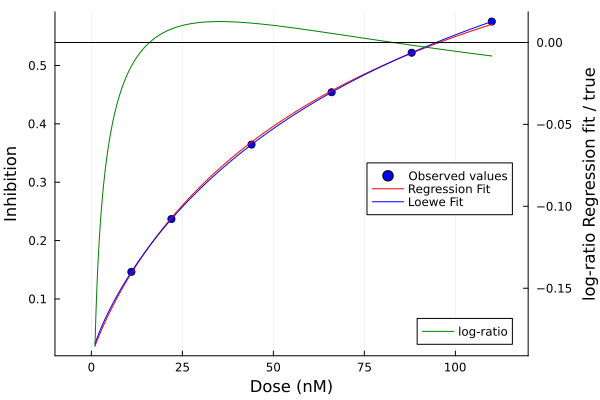
\includegraphics[width = 0.65\textwidth]{figs/CI-bias-dose-response.png}
        \end{center}
        ``Sometimes the [CombInd] values are $>3$ or much greater, especially at low effect levels...''
    }

    \only<3>{
        Then we would generate the following Inhibition-Combination Index plot:
        \begin{center}
            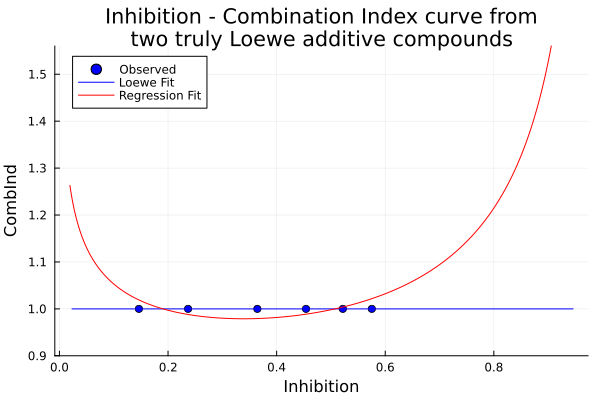
\includegraphics[width = 0.65\textwidth]{figs/CI-bias.png}
        \end{center}
        ``For anticancer or antiviral agents, synergy at high effect levels... is more relevant to therapy than at low effect levels...''
    }
\end{frame}

\begin{frame}{Chou-Tulalay Combination Index Example}
    \begin{center}
        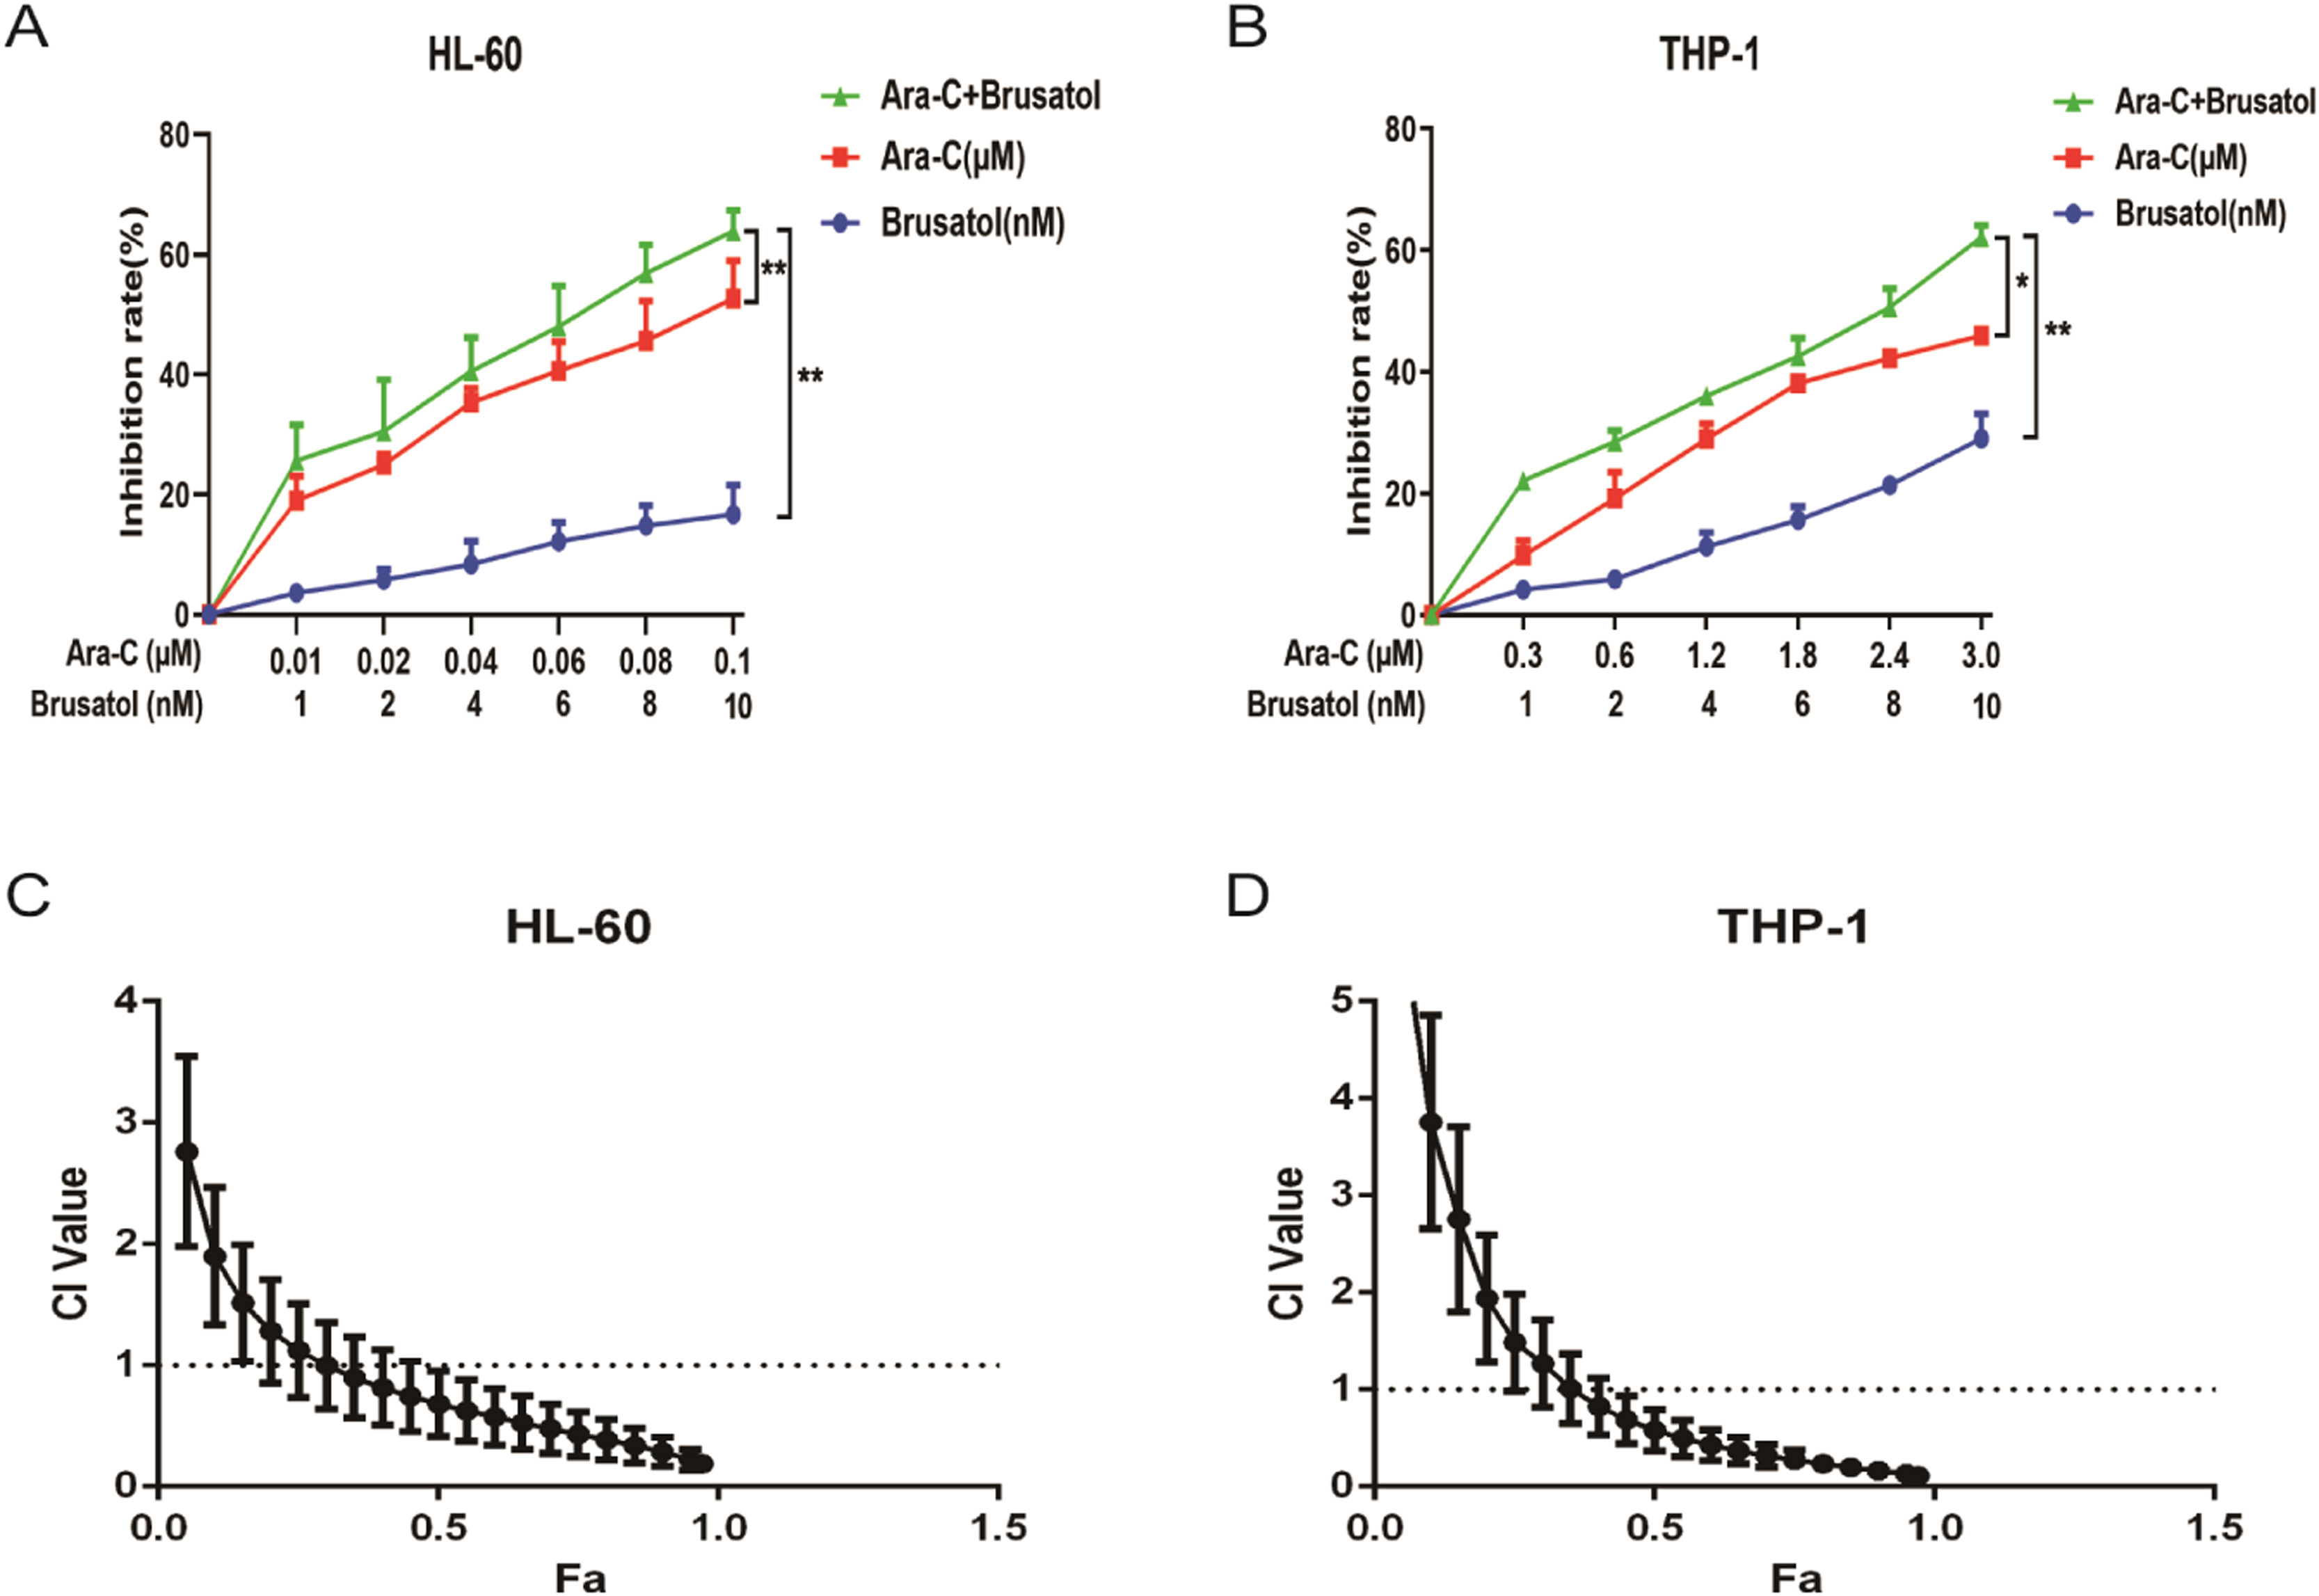
\includegraphics[width = 0.7\textwidth]{figs/ci-example.jpg}
        \hspace*{15pt}\hbox{\scriptsize Credit:\thinspace{\scriptsize\itshape Cheng et. al., 2012}}
    \end{center}
    Conclusion: Synergy is most highly expressed at 0.1$\mu$M Ara-C, 10nM Brusatol, so that dose was used in further experiments.
\end{frame}

\begin{frame}[t]{Chou-Tulalay Combination Index Example (cont'd.)}
    \begin{columns}
        \begin{column}{0.5\textwidth}
            \centering
            \large \underline{Brusatol + Ara-C}
            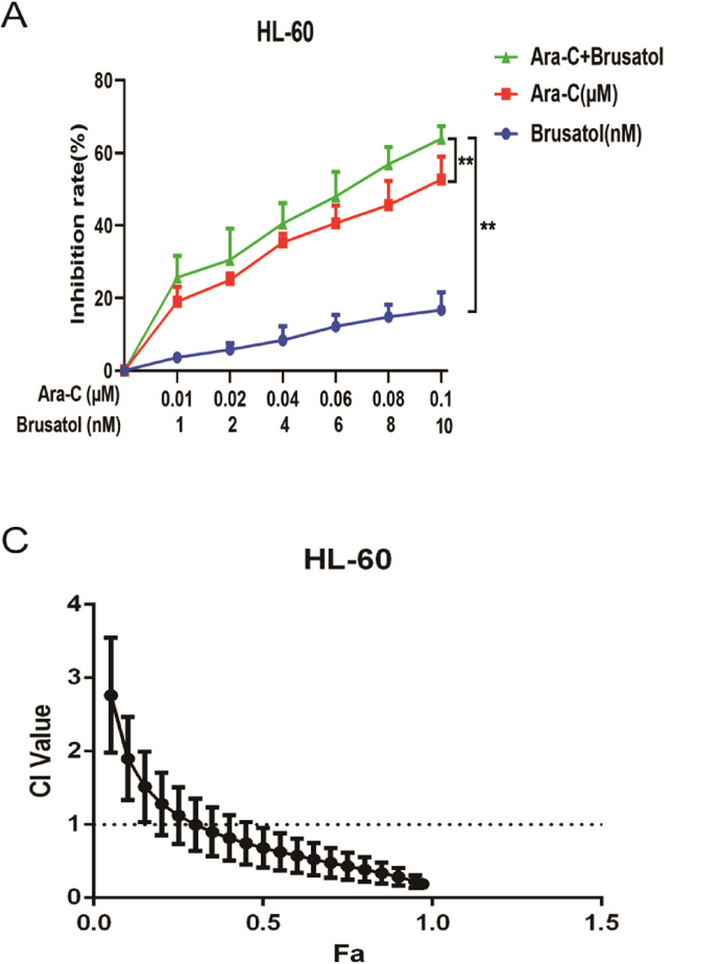
\includegraphics[width=0.9\textwidth, height = 0.7\textheight]{figs/brusatol-synergy-example.png}
        \end{column}
        \begin{column}{0.5\textwidth}
            \begin{figure}
                \centering
                \large \underline{``Toy'' Example}
                \begin{subfigure}{0.9\textwidth}
                    \centering
                    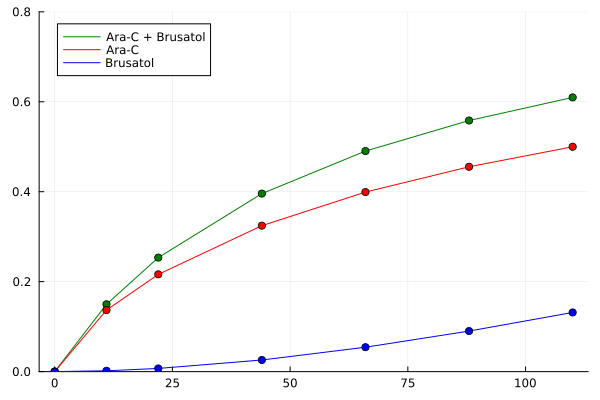
\includegraphics[width=0.9\textwidth, height = 0.35\textheight]{figs/my-brusatol.png}
                \end{subfigure}
                \begin{subfigure}{0.9\textwidth}
                    \centering
                    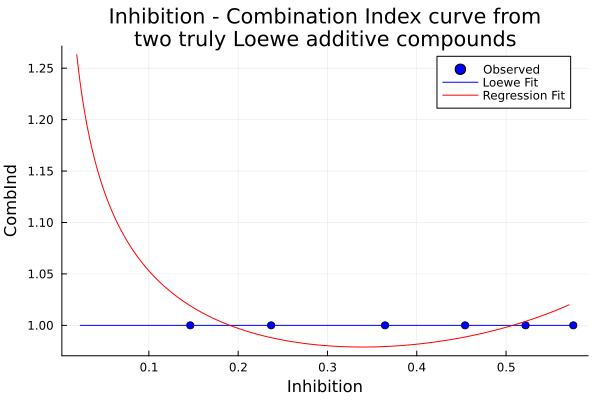
\includegraphics[width=0.9\textwidth, height = 0.35\textheight]{figs/CI-bias-nonlog.png}
                \end{subfigure}
            \end{figure} 
        \end{column}
    \end{columns}
\end{frame}

\begin{frame}[t]{Using Loewe Additivity}
    \begin{center}
        \alert{Only fit the curve once!}
        \noindent\makebox[\linewidth]{\rule{\textwidth}{0.4pt}}
    \end{center}
    \begin{columns}[c]
        \begin{column}[c]{0.4\textwidth}
            Eliminates double-fitting bias 
            \begin{itemize}
                \item \alert{Values} are compared to the additive curve
                \item Results are not dependent on range of doses tested
            \end{itemize}
        \end{column}
        \begin{column}[c]{0.4\textwidth}
            Can only get CombInd values at observed effects
            \begin{itemize}
                \item Can't use, say, CombInd$_{50}$
                \item How do we compare different combinations?
            \end{itemize}
        \end{column}
    \end{columns}
        % \vfill
    \begin{center}
        \noindent\makebox[\linewidth]{\rule{\textwidth}{0.4pt}}
        \only<2>{Aggregate results over doses tested}
    \end{center}
\end{frame}

\begin{frame}{Synergy Finder}
    \textit{R} package
    \begin{itemize}
        \item Calculates Loewe synergy scores \alert{without} fitting a second multi-compound dose-response curve
        \item Performs bootstrapping to get dose-level confidence intervals
        \item Aggregates values to get confidence interval for mean score \alert{over all dose combinations}
    \end{itemize}
\end{frame}

\begin{frame}{Loewe Synergy Score}
    \begin{Definition}
        Let $y_{\lambda, D}$ be an observation of $f_{AB, \lambda}(D)$, and let $y_{Loewe, \lambda, D}$ be the fitted value of $f_{AB, \lambda}(D)$ given some monotherapeutic dose-response data and model.
        Then the \alert{Loewe synergy score} is \[
            S_{Loewe, \lambda, D} = y_{\lambda,D} - y_{Loewe, \lambda, D}.
        \]
    \end{Definition}
\end{frame}

\begin{frame}{Loewe Synergy for Atovaquone-Brusatol}
    \centering
    \only<1>{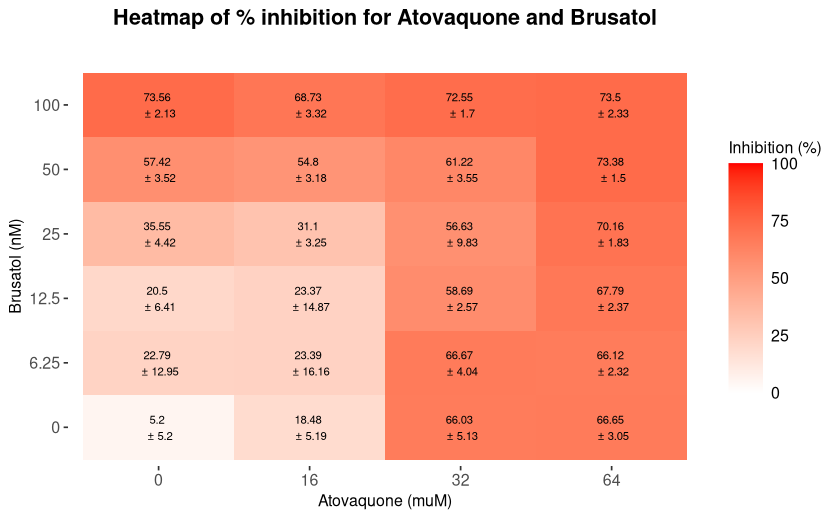
\includegraphics[width=0.9\textwidth]{figs/response-heatmap.png}}
    \only<2>{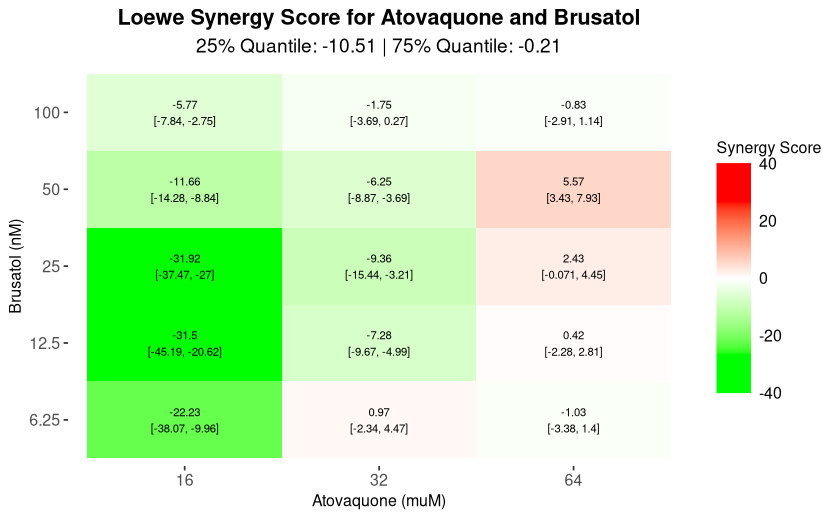
\includegraphics[width=0.9\textwidth]{figs/loewe-heatmap.png}}
\end{frame}

\begin{frame}{Other Synergy Scores}
    Synergy Finder also includes the three other synergy scores used by DrubCombDB
    \begin{itemize}
        \item Bliss additivity: Cell death as a result of one drug is statistically independent of cell death as a result of the other
        \item ZIP additivity: After some initial effect, the presence of one drug has no effect on the dose-response curve of the other
        \item HSA additivity: The drug combination will perform as well as the highest performing of its constituent parts
    \end{itemize}
\end{frame}

\begin{frame}[t]{Bliss Additivity}
    \begin{definition}[Bliss Additivity]
        Drugs $A$ and $B$, in ratio $\lambda$ : $(1 - \lambda)$ are \alert{Bliss additive} at dose $D$ if \[
            f_{AB, \lambda}(D) = f_A(\lambda D) + f_{B}((1 - \lambda) D) - f_A(\lambda D)\times f_{B}((1 - \lambda) D).
        \]
        
    \end{definition}
    \vfill

    \begin{itemize}
        \item \alert{Fails} Sham-combination experiment 
        \item Measurements are not actual observations of death/no death
        \item Does not even require monotherapeutic dose-response fitting
    \end{itemize}
\end{frame}

\begin{frame}{Bliss Additivity for Atovaquone and Brusatol}
    \centering
    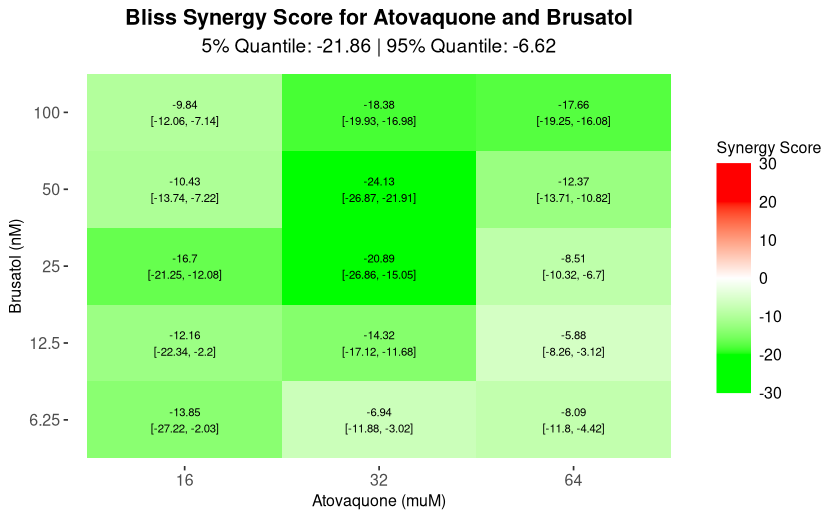
\includegraphics[width=0.9\textwidth]{figs/bliss-heatmap.png}
\end{frame}

\begin{frame}{ZIP Additivity}
    \begin{definition}[ZIP additivity]
        Let $A$ and $B$ be compound, where $A$ has hill coefficient $n_A$ and median effect dose $D_{mA}$. 
        For simplicity, assume drugs $A$, $B$, both follow MEE's. 
        Let
        \[
            f_A(D | B = d_b) = f_{AB}(D, d_b).
        \]
        $A$ and $B$ are \alert{ZIP additive} if 
        \[
            f_A(D | B = d_b) = \alert{f_B(d_b)} + \frac{1 - \alert{f_B(d_b)}}{1 + \left(\frac{D}{D_{mA}}\right)^{-n_A}}.
        \]
    \end{definition}
    \begin{itemize}
        \item ``Combines'' Loewe and Bliss additivity
        \item ZIP synergy score \alert{passes} sham-combination experiment 
        \item $f_{AB}(d_a, d_b) = f_A(d_a) + f_B(d_b) - f_A(d_a)f_B(d_b)$
    \end{itemize}
\end{frame}

\begin{frame}{ZIP Additivity for Atovaquone and Brusatol}
    \centering
    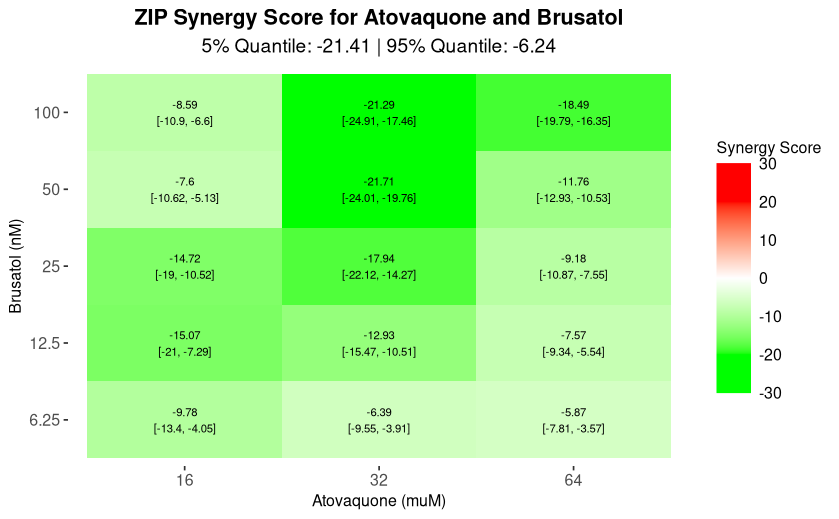
\includegraphics[width=0.9\textwidth]{figs/zip-heatmap.png}
\end{frame}

\begin{frame}{HSA Additivity}
    \begin{definition}[HSA additivity]
        We say that compounds $A$ and $B$ are \alert{HSA additive} if
        \[ 
            f_{AB}(d_a, d_b) = \max\{f_A(d_a),f_B(d_b)\}.
        \]
    \end{definition}

    \begin{itemize}
        \item Provides a \alert{lower-bound} for additivity definitions
        \item Not very useful for determining synergy 
        \item Very handy for determining antagonism
        \item May be preferred when one drug has little effect
    \end{itemize}
\end{frame}

\begin{frame}{HSA Additivity for Atovaquone and Brusatol}
    \centering
    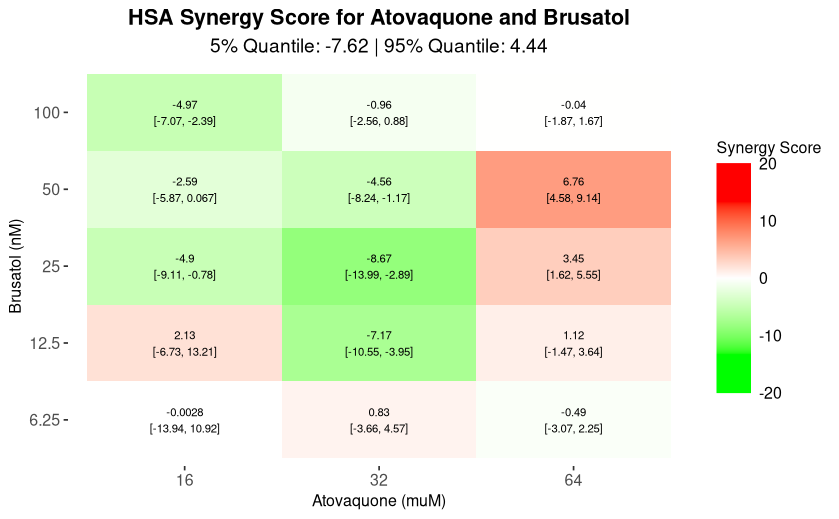
\includegraphics[width=0.9\textwidth]{figs/hsa-heatmap.png}
\end{frame}

\begin{frame}{Holistic Synergy Inference}
    \begin{itemize}
        \item Many more definitions of synergy exist \begin{itemize}
            \item Non-parametric, e.g., Hand 
            \item Parametric, e.g., BRAID / Linear models
        \end{itemize}
        \item No clear ``winner'', people have their favorites
        \item Best to report multiple, and make inferences holistically
    \end{itemize}
\end{frame}
    
\begin{frame}{Constant Ratio Dose-Response Curves}
    \begin{figure}[b]
        \centering
        \begin{subfigure}{0.5\textwidth}
            \centering
            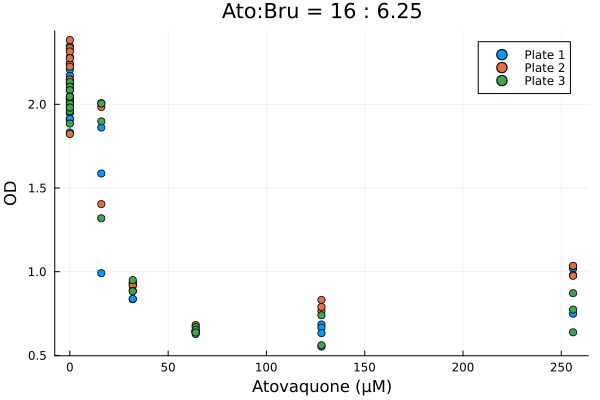
\includegraphics[width=0.9\textwidth]{figs/constant_rate_16to6.25.png}
        \end{subfigure}%
        \begin{subfigure}{0.5\textwidth}
            \centering
            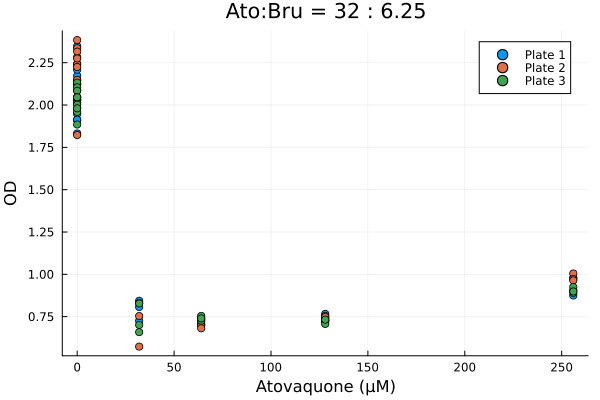
\includegraphics[width=0.9\textwidth]{figs/constant_rate_32to6.25.png}
        \end{subfigure}
        \begin{subfigure}{0.5\textwidth}
            \centering
            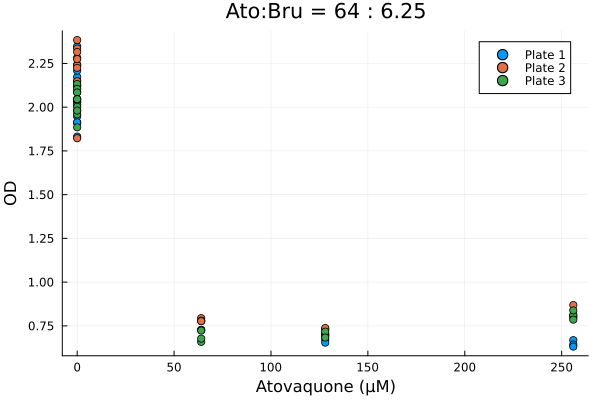
\includegraphics[width=0.9\textwidth]{figs/constant_rate_64to6.25.png}
        \end{subfigure}%
        \begin{subfigure}{0.5\textwidth}
            \centering
            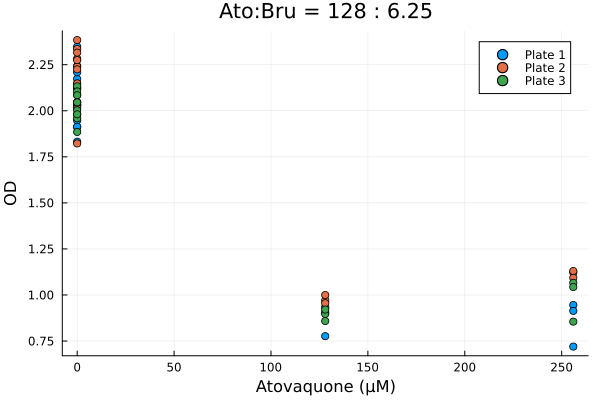
\includegraphics[width=0.9\textwidth]{figs/constant_rate_128to6.25.png}
        \end{subfigure}
    \end{figure}
\end{frame}


\begin{frame}{Synergy Finder (cont'd.)}
    For each observed $\lambda, D$, assume replicates $y^k\sim N(\bar y, \hat\sigma^2)$.
    \begin{itemize}
        \item Draw $B$ bootstrap samples $y^{k\prime}$
        \item Re-estimate monotherapeutic dose-response curves 
        \item Calculate Loewe synergy scores $(s_{\lambda, D}^b)_{b=1}^B$ 
        \item Calculate average synergy score as $s_b^\prime = {\rm mean}\{s_{\lambda, D}^b \mid \lambda\in(0,1)\}$
    \end{itemize}
    Obtain confidence intervals / $p$-values for each dose, and the average over all doses
\end{frame}


\end{document}
